\documentclass[bibtotoc,liststotoc,BCOR=5mm,DIV=12]{scrbook}

% use this declaration to set specific page margins
%\usepackage[a4paper , lmargin = {2.7cm} , rmargin = {2.9cm} , tmargin = {2.7cm} , bmargin = {4.6cm} ]{geometry}
\usepackage[a4paper]{geometry}

\usepackage[english]{babel}
\usepackage{bibgerm}       		% german references
\usepackage[T1]{fontenc} % german characters
\usepackage{graphicx} 				% it's recommended to use PDF images but you can use JPG or PNG as well
\usepackage{url}           		% format URLs
\usepackage{hyperref} 				% create hyperlinks
\usepackage{listings, color}	% for source code
\usepackage{subfig}						% two figures next to each other (example: figure 3a), figure 3b)
\usepackage{scrlayer-scrpage}					% header and footer line
\usepackage{todonotes}
\usepackage{multicol}
% header and footer line - no header & footer line on pages where a new chapter starts
\pagestyle{scrheadings}
\ohead{Design, Implementation and Evaluation of\newline Zero Knowledge Rollups using the ZoKrates Toolbox}
\ihead{Dott. De Tomasi Andrea}
\ofoot[]{\thepage}
\ifoot{Master Thesis, TU Berlin, ISE Department, 2023}

% set path where images are stored
\graphicspath{{./img/}}


\begin{document}
% ---------------------------------------------------------------
\frontmatter
    \thispagestyle{empty}
\begin{center}

\vspace*{1cm}
{\LARGE \textbf{Technische Universität Berlin}}

\vspace{0.5cm}

{\large Information Systems Engineering\\[1mm]}

Fakultät IV\\
Einsteinufer 17\\
10587 Berlin\\
https://www.tu.berlin/ise\\

\vspace*{1cm}

\includegraphics[width=4cm]{tu_logo}

\vspace*{1.0cm}

{\LARGE Master Thesis}\\

\vspace{1.0cm}
{\LARGE \textbf{Design, Implementation and Evaluation of}}\\
\vspace*{0.2cm}
{\LARGE \textbf{Zero Knowledge Rollups using the ZoKrates Toolbox}}\\
\vspace*{0.2cm}
{\LARGE \textbf{}}\\
\vspace*{1.0cm}
{\LARGE Dottore De Tomasi Andrea}
\\
\vspace*{0.5cm}
Matriculation Number: 478814\\
11.10.2023\\
\vspace*{1.2cm}

Supervised by\\
Prof. Dr.-Ing Stefan Tai\\
Prof. Dr. Florian Tschorsch\\
\vspace*{0.2cm}
Assistant Supervisor\\
M.Sc. Jonathan Heiß
\end{center}

    \thispagestyle{empty}
    \cleardoublepage
    
    
    \include{./misc/self-assertion} 
    \thispagestyle{empty}
    \cleardoublepage

    \thispagestyle{empty}

\begin{flushright}
    % \slshape
    \textsl{`Life is like a box of chocolates\\You never know what you're gonna get'}
    \\
    \medskip
    --- Forrest Gump
\end{flushright}


\bigskip

\begin{center}
    \textbf{Acknowledgements}
\end{center}

\noindent I want to thanks my parents Fabio and Daniela, for always supporting me in my choices, encouraging me to do what I was most interested in and stimulated without having fears or worries.

% \noindent \textit{Desidero ringraziare i miei genitori Fabio e Daniela, per avermi sempre supportato nelle mie scelte, incoraggiandomi a fare ciò che più mi interessava e stimolava senza avere paure o preoccupazioni.}


% \noindent \textit{Desidero inoltre ringraziare mia sorella Jenny che è stata sempre presente in caso di qualsiasi bisogno.}


% \noindent \textit{Ringrazio i miei amici, compagni di mille avventure ed esperienze, con cui sono cresciuto e maturato sin dai tempi delle scuole superiori, sperando di poter mantenere questi legami a lungo nel tempo.}
    \thispagestyle{empty}
    \cleardoublepage
    
    
    \thispagestyle{empty}
\vspace*{1.0cm}

\begin{center}
    \textbf{Abstract}
\end{center}

\vspace*{0.5cm}

\noindent
Blockchains faced an increase of usage in recent years, posing new challenges to the scalability and efficiency of the system. Several congestion incidents have happened in the past, making blockchains slow and incredibly costly. To mitigate these episodes some internal modifications of the blockchains have been proposed, known as Layer 1 solutions. After being revealed quite inefficient some other type of enhancements that exploit resources outside the blockchain have been studied, called Layer 2 solutions. Between those Layer 2 solutions there are rollups: they consist in executing a bunch of transactions outside the blockchain, and sending just the result of the rollup computation to the blockchain. This approach allows just one blockchain interaction per group of transaction instead of one per every transaction. This allows to save on fees and reduce the congestion on the blockchain.

One type of Rollups are Zero-Knowledge Rollups (Zk-Rollups): they allow executing a rollup and send a proof of correct execution to the blockchain, that will verify it and include the rollup results in its state. One problem with this type of rollup is they are very resource demanding for the Layer 2 system. To ease the creation of Zero-Knowledge programs some toolbox are available: one of them is ZoKrates, developed at the Technical University of Berlin.

This master thesis proposes a Zk-Rollup system written using the ZoKrates toolbox, that can be applied to the vast majority of blockchains with little modifications. The Rollup System is deployed for the testing and development on the Tezos Blockchain. The system shows its capability on handling different types of tokens, like in the case of an NFT marketplace and on saving on fees, while remaining usable during congestions. It resulted also to be resource-efficient, allowing to run it on a wide range of hardware.


% This template is intended to give an introduction of how to write diploma and master thesis at the chair 'Architektur der Vermittlungsknoten' of the Technische Universität Berlin. Please don't use the term 'Technical University' in your thesis because this is a proper name. 
% \\
% \\
% On the one hand this PDF should give a guidance to people who will soon start to write their thesis. The overall structure is explained by examples. On the other hand this text is provided as a collection of LaTeX files that can be used as a template for a new thesis. Feel free to edit the design.
% \\
% \\
% It is highly recommended to write your thesis with LaTeX. I prefer to use Miktex in combination with TeXnicCenter (both freeware) but you can use any other LaTeX software as well. For managing the references I use the open-source tool jabref. For diagrams and graphs I tend to use MS Visio with PDF plugin. Images look much better when saved as vector images. For logos and 'external' images use JPG or PNG. In your thesis you should try to explain as much as possible with the help of images.
% \\
% \\
% The abstract is the most important part of your thesis. Take your time to write it as good as possible. Abstract should have no more than one page. It is normal to rewrite the abstract again and again, so  probaly you won't write the final abstract before the last week of due-date. Before submitting your thesis you should give at least the abstract, the introduction and the conclusion to a native english speaker. It is likely that almost no one will read your thesis as a whole but most people will read the abstract, the introduction and the conclusion.
% \\
% \\
% Start with some introductionary lines, followed by some words why your topic is relevant and why your solution is needed concluding with 'what I have done'. Don't use too many buzzwords. The abstract may also be read by people who are not familiar with your topic.
    \thispagestyle{empty}
    \cleardoublepage
    
    \tableofcontents
    \thispagestyle{empty}
    
    %\todo[inline]{talk to your supervisor if this is needed}
    \listoffigures
    \thispagestyle{empty}
    
    
% --------------------------------------------------------------

\mainmatter % comment single chapters for faster compilation

    \chapter{Introduction}\label{cha:chapter1}

This chapter provides an overview of the motivation, context, and objectives of the thesis.

\section{Motivation}\label{sec:moti}

In recent years, blockchain technology has witnessed remarkable growth, with the introduction of Bitcoin in 2008 \cite{nakamoto_bitcoin_2008} marking the emergence of a decentralized, distributed ledger concept. Since then, numerous blockchains with unique features have been developed, gaining widespread popularity.

As the popularity of blockchains continues to rise, many companies are exploring the technology's potential and attracting new users. Predictions indicate exponential growth in the blockchain space in the coming years \cite{noauthor_global_nodate}. However, this growth presents a challenge due to the limited scalability offered by current blockchains. For instance, Ethereum, one of the most popular blockchains, currently faces a transaction processing limit of only 15 transactions per second (TPS).

The necessity for blockchain scalability has been recognized by the community, especially evident when Ethereum transaction fees reached an average of \$70 in 2020\footnote{\url{https://ycharts.com/indicators/ethereum_average_transaction_fee}} due to the high volume of submitted transactions and consequent congestion of the network. This issue is not unique to Ethereum, as other blockchains also experience similar problems. Vitalik Buterin's `Scalability Trilemma' assert that achieving scalability, security, and decentralization simultaneously in a distributed system, such as blockchains, is a challenging task\footnote{\url{https://ethereum.org/en/roadmap/vision/}}.

\section{Objective}\label{sec:objective}

The objective of this thesis is to address the issue of limited scalability and high fees in blockchains. A crucial factor that constrains the number of transactions in a block is gas limit. The gas limit serves as a hard limit on the computational work that can be performed within a block, measured in gas units. Each transaction and contract interaction, in fact, consumes gas, so gas limit determines the maximum amount of computational availability.

The gas limit mechanism is essential for preventing infinite loops in a smart contract execution and defending against denial-of-service attacks. It's also necessary to ensure that a minimal number of transactions can be included in the block. However, it can also inhibit the proper execution of a program that intentionally involves extended computations \cite{wood_ethereum_nodate}.

Enhancing the blockchain's throughput is also directly impacted by the block size, as increasing its size can increase the system's capacity. Nonetheless, a thorough analysis of the consequences of enlarging the block size is necessary, as arbitrary increases can lead to negative effects. For instance, large block sizes may cause network congestion, slower propagation speeds, and an increase in the number of stale blocks—blocks that are not included in the longest chain due to conflicts or concurrency—posing potential security risks \cite{gervais_security_2016}.

This thesis proposes a solution to the scalability problem by introducing a new block-chain Layer that lives on top of the original blockchain. This is called a Layer 2 solution (L2). This second Layer is entirely run by nodes that are not involved in computing or verifying Layer 1 transactions. This way we are not constrained by limitations imposed by the chain, like the gas limit or block size, but we are free to use a lot more computational power. Rollups, a Layer 2 solution, in fact inject into the blockchain only the result of the computations performed outside the chain, making use of the unconstrained computational availability offered on L2. With this approach it should be possible to achieve higher throughput when congestion occurs and lower transaction fees.

This thesis poses three key milestones for achieving the objective of obtaining a functional and efficient Rollup System. These primary objectives can be summarized as follows:
\begin{itemize}
    \vspace{-0.11in}
    \item finalize the zk-rollup project upon which this system is built;
          \vspace{-0.11in}
    \item conduct an evaluation, enhancement, and benchmark of the rollup system.
          \vspace{-0.11in}
    \item create and build a prototype customized to run a NFT marketplace.
\end{itemize}\

A deeper explanation about problem statements and research questions is given in Chapter \ref{sec:4_problemrefinement}.

\section{Structure\label{sec:structure}}

\todo[inline]{Change}

This section gives a brief introduction into the main chapters of this thesis.
\\
\\
\textbf{Chapter \ref{cha:chapter2}} analyzes the current state of the art in the field of blockchain scalability and presents the most relevant related work including the project this thesis is based on.
\\
\\
\textbf{Chapter \ref{cha:chapter3}} analyzes the research question and the requirements for the Rollup System.
\\
\\
\textbf{Chapter \ref{cha:chapter4}} describes the architecture of the Layer 1 and Layer 2 components. It also describes the communication between the two layers.
\\
\\
\textbf{Chapter \ref{cha:chapter5}} describes the implementation part of the Rollup System.It shows the components and the technologies used to build the system. It also describes the challenges faced during the development.
\\
\\
\textbf{Chapter \ref{cha:chapter6}} shows the tests performed and the results obtained. It also shows the limitations of the system and the possible future improvements.
\\
\\
\textbf{Chapter \ref{cha:chapter7}} summarizes the work done and the challenges faced. It presents the conclusions and the future work to improve the system.

    \chapter{State of the Art \& Related Work}
\label{cha:chapter2}

This chapter provides an overview of the prominent solutions in the realm of blockchain scalability and introduces the foundational project upon which this thesis is built.

\section{Scalability Approaches}
Various strategies are being explored to enhance blockchain scalability. Some are already operational, while others are in the research stage. These strategies broadly fall into two categories: Layer 1 and Layer 2 solutions \cite{tyagi_study_2021,thibault_blockchain_2022}. Layer 1 solutions focus on boosting blockchain scalability through means like enlarging block sizes or implementing Sharding. In contrast, Layer 2 solutions endeavor to scale the blockchain by relocating computation off-chain. Noteworthy examples of Layer 2 solutions encompass State Channels, Sidechains, and Rollups, as illustrated in Figure \ref{fig:2_scalingSolutions}.

The prevailing trajectory for blockchain scalability involves the adoption of Layer 2 solutions. This course of action is being embraced by a significant portion of the Ethereum community \cite{neiheiser_practical_2023}.

\begin{figure}[ht]
  \centering
  \includegraphics[width=0.95\columnwidth]{2_scalingSolutions.jpg}
  \caption[Scaling Solutions]{Principal scaling solutions for Layer 1 and Layer 2\footnotemark}  
  \label{fig:2_scalingSolutions}
\end{figure} 
\footnotetext{\url{https://medium.com/token-terminal/a-primer-on-ethereum-l2-scaling-techniques-17ac437891b1}}

\subsection{Zk-Rollups}
\label{sec:2_zkRollups}
Zk-Rollups represent a Layer 2 approach that leverages zero-knowledge proofs to conduct computation off-chain. Post-computation outcomes and a proof of verifiably correct execution are transmitted to the blockchain's smart contract. The smart contract then verifies the proof before incorporating the results onto the blockchain \cite{tyagi_study_2021}.

Figure \ref{fig:2_zkRollup_schema} outlines the Zk-Rollup paradigm. An user initiates a transaction with the off-chain node. The node processes the transaction batch, using the state fetched from the blockchain, and relays results and proof to the smart contract. Following proof validation, the new account balance list is recorded on the blockchain.

\begin{figure}[ht]
  \centering
  \includegraphics[width=0.95\columnwidth]{2_zkRollup_architecture.png}
  \caption[Zk-Rollup Schema]{General schema of a Zk-Rollup\cite{ise_department_tub_material_nodate}}  
  \label{fig:2_zkRollup_schema}
\end{figure}

\subsection{ZoKrates}
ZoKrates is a toolbox for zkSNARKs on Ethereum: it allows developers to write zero-knowledge proofs in a high-level programming language and generate trusted setup parameters and zero-knowledge proofs \cite{eberhardt_ZoKrates_2018}.

\todo[inline]{explain ZoKrates}

\section{ADSP Project: Scaling Tezos Blockchain with Zk-Rollups}
In the Winter Semester 2022/2023 at the University of Berlin, I collaborated with the ADSP (Advanced Distributed Systems Prototype) group on a project. The project's objective was to scale the Tezos blockchain using Zk-Rollups through the ZoKrates toolbox.

The group partially achieved the project's objectives, creating a proof of concept. The system architecture features Layer 1 and Layer 2 components: Layer 1 includes two smart contracts for state management and proof verification; Layer 2 encompasses a node executing transactions within the ZoKrates program, generating proofs for the smart contract. Figure \ref{fig:2_general_rollup_architecture} offers an overview of the entire system.

\begin{figure}[ht]
  \centering
  \includegraphics[width=0.95\columnwidth]{2_drawings-adsp_rollup_architecture.png}
  \caption[Zk-Rollup Architecture]{General Zk-Rollup architecture}  
  \label{fig:2_general_rollup_architecture}
\end{figure}

The Zk-Rollup execution process unfolds as follows:
\begin{enumerate}
    \item A user dispatches a transaction to the off-chain node, managed by a NodeJS server (the manager);
    \item The manager logs the transaction in a transaction queue;
    \item Once three transactions accumulate, the node processes the transaction batch, spawning the ZoKrates executor;
    \item The manager fetches the current state from the Tezos Zk-Rollup smart contract;
    \item The ZoKrates executor processes the ZoKrates program with the transaction batch and the current state as input;
    \item The ZoKrates executor generates a proof and new balance list, transmitting them to the NodeJS server;
    \item The NodeJS server converts ZoKrates outputs into a Tezos-compatible format;
    \item Converted outputs are dispatched to the Tezos Zk-Rollup smart contract;
    \item The smart contract forwards the proof to the verifier smart contract;
    \item The verifier smart contract verifies the proof, communicating the result to the contract;
    \item If the proof is verified, the new balance list is stored in the Zk-Rollup contract's blockchain storage.
\end{enumerate}

Figure \ref{fig:2_drawings-adsp_sequence_general.png} illustrates the sequence of events in the Zk-Rollup execution process.

\begin{figure}[ht]
  \centering
  \includegraphics[width=1\columnwidth]{2_drawings-adsp_sequence_general.png}
  \caption[Scaling Solutions]{Sequence diagram of the Zk-Rollup execution process.}  
  \label{fig:2_drawings-adsp_sequence_general.png}
\end{figure} 

\subsection{Developed Components}
The team successfully implemented the Zk-Rollup \textit{Verify} entrypoint within the \textit{Zk-Rollup contract}, along with the \textit{NodeJS Manager}. Additionally, the storage mechanism was correctly executed.

The ZoKrates program was partially developed, including:
\begin{itemize}
    \item Verification of account inclusion in the rollup system;
    \item Verification of sufficient balance in sender account;
    \item Transaction execution;
    \item Generation of new balance merkle tree root, balance list, and proof.
\end{itemize}

The generation of the Merkle tree root is accomplished through the algorithm described below. This process utilizes the SHA2-256 hash function with automatic zero-padding. The algorithm incorporates pre-calculated values for the Merkle tree depth and the number of leaf nodes.

\textbf{Algorithm 1: Merkle Tree Root Generation}
\begin{lstlisting}[language=Python]
for i in 0...TREE_DEPTH {
  step_size = 2 ** (i + 1)
  step_number = LEAFS_NUM / step_size
  for j in 0...step_number {
    leftIndex = j * step_size
    rightIndex = leftIndex + step_size / 2
    leafs[leftIndex] = hash(
        leafs[leftIndex],
        leafs[rightIndex]
    )
  }
}
return leafs[0]
\end{lstlisting}

\subsection{Pending Components\label{subsec:pendingcomponents}}
Numerous aspects of the project remain unfinished, including:
\begin{itemize}
  \item Registration entrypoint;
  \item Deregistration entrypoint;
  \item Deposit entrypoint;
  \item Withdrawal entrypoint;
  \item Integration of signature checks within the ZoKrates program;
  \item Addressing the double spending issue;
  \item System optimization.
\end{itemize}
Furthermore, the project lacks a benchmarking study, a security analysis, and a cost comparison with alternative scaling solutions and Layer 1.

\todo[inline]{Provide a more comprehensive analysis of the project's state of the art.}

\section{Other Zk-Rollup Implementations}
Numerous Zk-Rollup implementations exist, particularly for Ethereum. The implementation discussed in \cite{dinh_implementation_2023} shares similarities with the ADSP project's approach. However, it lacks considerations for system scaling and handling multiple token types. Another example is Polygon Zero\footnote{\url{https://polygon.technology/blog/introducing-plonky2}}, which facilitates parallel execution of transactions on L2. This system blends STARK and SNARK, differing from the approach outlined in this thesis.

\section{Zk-Rollup Reviews}
Several studies have assessed the viability and performance of the Zk-Rollup system. \cite{capko_state_2022} offers an overview of prevalent zero-knowledge proofs. The ZoKrates Toolbox, utilized by the ADSP project, employs SNARK, which requires a trusted setup phase—a potential drawback compared to Transparent zk-SNARK \cite{zhou_overview_2022}. \cite{neiheiser_practical_2023} highlights the scalability bottleneck L2 solutions face due to slow L1, constraining them below theoretical L2 throughput. \cite{starkware_fractal_2021} proposes L3 to circumvent this issue.

\section{Alternative L2 Solutions}
Several Layer 2 strategies exist to scale blockchains. A brief overview follows.

Plasma: Plasma facilitates off-chain transaction processing through child chains or sidechains, connected to the main blockchain for security. Plasma chains expedite transactions but necessitate dispute resolution for potentially fraudulent actions \cite{thibault_blockchain_2022}. OMG Network\footnote{\url{https://docs.omg.network}} exemplifies a network employing Plasma.

State Channels: Off-chain payment channels, like state channels, enable direct user transactions without main blockchain interaction. They suit use cases like micropayments and gaming, affording fast, economical transactions \cite{negka_blockchain_2021}. Perun\footnote{\url{https://perun.network/wp-content/uploads/Perun2.0.pdf}} serves as an instance of state channel implementation.

Optimistic Rollups: This type assumes transaction validity, necessitating verification only during disputes. It combines swifter transactions with main blockchain arbitration \cite{thibault_blockchain_2022}.

    \chapter{Related Work\label{cha:chapter3}}

This chapter gives a look at the main ideas in blockchain scalability and introduces the core project on which this thesis is based.

\section{Scalability Approaches}
Various strategies are being explored to enhance blockchain scalability. Some are already operational, while others are in the research stage. These strategies broadly fall into two categories: Layer 1 and Layer 2 solutions \cite{tyagi_study_2021,thibault_blockchain_2022}. Layer 1 solutions focus on boosting blockchain scalability through means like enlarging block sizes or implementing Sharding. In contrast, Layer 2 solutions attempt to scale the blockchain by relocating computation off-chain. Noteworthy examples of Layer 2 solutions are State Channels, Sidechains, and Rollups, as illustrated in Figure \ref{fig:3_scalingSolutions}.

The common path for making blockchains handle more transactions is to use Layer 2 solutions. Many members of the Ethereum community are following this approach \cite{neiheiser_practical_2023}.

\begin{figure}[ht]
  \centering
  \includegraphics[width=0.95\columnwidth]{2_scalingSolutions.jpg}
  \caption[Scaling Solutions]{Principal scaling solutions for Layer 1 and Layer 2\footnotemark}  
  \label{fig:3_scalingSolutions}
\end{figure} 
\footnotetext{\url{https://medium.com/token-terminal/a-primer-on-ethereum-l2-scaling-techniques-17ac437891b1}}

\section{Zk-Rollups}
\label{sec:2_zkRollups}
Zero-Knowledge Rollups represent a Layer 2 scaling approach that takes advantage of capabilities of zero-knowledge proofs to facilitate off-chain computation. This strategy aims to alleviate the scalability limitations of blockchains by shifting most of the computational work away from the main chain while still maintaining the security and trustless nature of the system. In the context of Zk-Rollups, computation is executed off-chain, and the outcomes of these computations, accompanied by a proof of verifiably correct execution, are transmitted to the corresponding smart contract on the blockchain \cite{tyagi_study_2021}.

Figure \ref{fig:3_zkRollup_schema} illustrates the fundamental steps of the Zk-Rollup, explained by this sequence list:
\begin{enumerate}
  \item \textbf{Transaction Initiation:} Users initiate transactions with an off-chain processing node. This node is responsible for collecting and batching multiple transactions together;
  \item \textbf{Off-chain Computation:} The processing node performs computations off-chain, fetching the current state from the underlying blockchain;
  \item \textbf{Proof Transmission:} After processing the transaction batch, the node generates a proof attesting to the validity of the computations performed. This proof, along with the resulting transaction outcomes, is then transmitted to the blockchain's smart contract;
  \item \textbf{Proof Verification:} The smart contract receives the proof and checks its correctness. This step involves cryptographic operations to confirm that the computation was executed correctly and honestly;
  \item \textbf{State Update:} If the proof verification is successful, the smart contract updates its internal state on the blockchain to store the outcomes of the off-chain computation. This ensures that the blockchain remains in sync with the results of the computations performed in the Layer 2 solution.
\end{enumerate}

\begin{figure}[ht]
  \centering
  \includegraphics[width=0.95\columnwidth]{2_zkRollup_architecture.png}
  \caption[Zk-Rollup Schema]{General schema of a Zk-Rollup\cite{ise_department_tub_material_nodate}}  
  \label{fig:3_zkRollup_schema}
\end{figure}

\subsection{Zk-Rollup Implementations}
Some other Zk-Rollup implementations exist, particularly for Ethereum. The implementation discussed in \cite{dinh_implementation_2023} shares similarities with the ADSP project's approach. However, it lacks considerations for system scaling and handling multiple token types. Another example is Polygon Zero\footnote{\url{https://polygon.technology/blog/introducing-plonky2}}, which facilitates parallel execution of transactions on L2. This system blends STARK and SNARK, differing from the approach outlined in this thesis. \cite{rybakken_intmax2_2023} presents an innovative approach to Zk-Rollup featuring stateless and decentralized block production, trying to limit the data stored on chain and moving the computations to the client-side. However, this approach follows a different path from the one presented in this thesis, which uses a more classic approach with a centralized smart contract and a decentralized node. \cite{liu_pianist_2023} Presents an innovative solution to ZK-Rollup limited scalability, using Plonk as proof system, and splitting the proving work between multiple nodes. This approach demonstrates a promising path to improve ZK-Rollup scalability, but differs from this thesis' approach, which uses a single node to perform the proving work with ZoKrates.

\subsection{Zk-Rollup Reviews}
Some studies have assessed the viability and performance of the Zk-Rollup system. \cite{capko_state_2022} offers an overview of prevalent zero-knowledge proofs. The ZoKrates Toolbox, utilized by the ADSP project, employs SNARK, which requires a trusted setup phase—a potential drawback compared to Transparent zk-SNARK \cite{zhou_overview_2022}. \cite{neiheiser_practical_2023} highlights the scalability bottleneck L2 solutions may face due to a possible slow L1, constraining them below theoretical L2 throughput. \cite{starkware_fractal_2021} proposes a new Layer 3 to overcome this issue.

\section{Alternative L2 Solutions}
Several Layer 2 strategies exist to scale blockchains, offering different approaches to address the scalability challenges faced by the blockchain. Below is a brief overview at some of these strategies.

\subsection{Plasma}
Plasma presents a dynamic off-chain transaction processing solution by introducing child chains or sidechains linked to the main blockchain. These connected chains, or Plasma chains, allow for a significant increase in transaction throughput by handling transactions off the main chain. This results in faster and more efficient transactions. However, Plasma's architecture introduces a challenge: the need for resolving disputes that may arise due to potentially fraudulent or incorrect actions on these child chains\cite{thibault_blockchain_2022}. This dispute resolution process is necessary to maintain the security and integrity of the system. An example of a project utilizing the Plasma approach is OMG Network\footnote{\url{https://docs.omg.network}}, which uses Plasma chains to enhance transaction scalability while relying on the security guarantees of the main Ethereum blockchain.

\subsection{State Channels}
State channels provide a different Layer 2 scaling solution that focuses on specific use cases such as micropayments and gaming interactions. These channels allow users to execute transactions directly with each other off the main blockchain, thus reducing the congestion on the main chain and enabling faster, low-cost transactions\cite{negka_blockchain_2021}. State channels work by locking a certain amount of cryptocurrency on the blockchain and then allowing multiple off-chain transactions to occur between participants. These transactions are only confirmed on the main chain when the participants want to close the channel or when a dispute arises. An example of a project implementing state channels is Perun\footnote{\url{https://perun.network/wp-content/uploads/Perun2.0.pdf}}, which offers a framework for efficient state channel networks.

\subsection{Optimistic Rollups \label{subsec:optimisticRollups}}
Optimistic Rollups offer a compromise between transaction speed and security by assuming the validity of transactions by default\cite{thibault_blockchain_2022}. In this approach, transactions are processed quickly on Layer 2, but the verification of these transactions is postponed to the main blockchain only if disputes arise. This optimistic assumption speeds up the entire transaction processing while maintaining the chance for arbitration if necessary. It's worth noting that the vast majority of transactions are expected to be valid, so this approach optimizes for the common case. Optimistic Rollups combine the efficiency benefits of Layer 2 scaling with the security guarantees of the main blockchain. A notable downside of this solution is the presence of a long waiting time for a transaction to be confirmed on the main chain. This is due to the need of waiting for the maximum possible duration during which a dispute could potentially be raised within a rollup execution, which is called the challenge period \cite{negka_blockchain_2021}. This challenge period can last for about one week before a transaction is confirmed on the main chain.



    \chapter{Design\label{cha:chapter4}}
This chapter presents the architectural design choices of the Rollup System. The Rollup System comprises Layer 1 components and Layer 2 components. The Layer 1 components encompass the Rollup smart contracts, while the Layer 2 components consist of the rollup programs and Web servers.

\section{Layer 1\label{sec:designlayer1}}
Layer 1 primarily consists of the rollup smart contracts. These contracts are divided into verifier contracts and a manager contract. The verifier contracts handle rollup proof verification, while the manager contract stores the rollup state and serves as a gateway, invoking the verifiers for proof verification.

\begin{figure}[htb]
  \centering
  \includegraphics[width=9cm]{4_Architecture-L1_general.png}
  \caption{Layer 1 Overview}
  \label{fig:layer1overview}
\end{figure}

This modular approach enables independent upgrades of verification contracts, addressing scenarios like bugs in L2 programs. New programs may require updated verification keys, leading to deployment of corresponding verifier contracts. By having dedicated entrypoints, the rollup contract can be updated to use new verifier contracts while leaving others unaffected, necessitating only one deployment.

Another advantage of separation is reduced gas consumption: each entrypoint loads only the necessary contract code into memory. With separate contracts, the rollup contract loads only the required verifier contract for proof verification, optimizing gas usage.

\subsection{Manager Contract\label{sec:designrollupcontract}}
The Manager contract is the primary interface of the Rollup System with the blockchain. Responsible for rollup state storage and verifier contract invocation, it indirectly stores transaction history in the blockchain.

Its entrypoints handle proofs from L2 programs: forwarding proofs to relevant verifiers, verifying them, and updating storage with new state. This process is illustrated in sequence diagram \ref{fig:layer1sequencediagram}.

\begin{figure}[ht]
  \centering
  \includegraphics[width=6cm]{4_Architecture-Sequence_general_L1.png}
  \caption{Layer 1 Sequence Overview}
  \label{fig:layer1sequencediagram}
\end{figure}

\paragraph{State}
Expanding the state defined in Section \ref{sec:2_zkRollups}, the Rollup System's state includes:
\begin{itemize}
  \item \textbf{Accounts Root}: Root of the Merkle Tree containing registered accounts;
  \item \textbf{Balances Root}: Root of the Merkle Tree containing account balances;
  \item \textbf{User Map}: Map of registered users, each represented by a user index, public key, and balance.
\end{itemize}

\paragraph{Entrypoints}
Multiple entrypoints optimize gas usage by loading only necessary code. Entrypoints for minimal functionality are:
\begin{itemize}
  \item \textbf{Register}: Register a new user;
  \item \textbf{Deregister}: Deregister a user;
  \item \textbf{Deposit}: Deposit funds;
  \item \textbf{Withdraw}: Withdraw funds;
  \item \textbf{Rollup}: Submit a rollup proof.
\end{itemize}

\subsection{Verifier Contracts\label{sec:designverifiercontracts}}
Verifier contracts validate rollup proofs. Each handles a specific proof type, invoked by the manager contract.

\textbf{Proof}: A structure with proof keys, public program inputs and program outputs.
\newline These contracts have no storage; they verify proofs through an entrypoint. A challenge arises with verification key sizes: large keys can hinder deployability and execution due to gas limits, as discussed in Section \ref{subsec:gasLimit}. 

\section{Layer 2\label{sec:designlayer2}}
Layer 2 consists of rollup programs and a Web server. Rollup programs generate zero-knowledge proofs, while the Web server exposes APIs for receiving transaction batches to be executed in a zero-knowledge context and sends proofs to the manager contract.

\begin{figure}[htb]
  \centering
  \includegraphics[width=13cm]{4_Architecture-L2_general.png}
  \caption{Layer 2 Overview}
  \label{fig:layer2overview}
\end{figure}

\subsection{Web Server\label{sec:designwebserver}}
The Web server provides APIs for zero-knowledge transaction execution. It calls rollup programs and awaits their completion, sending resulting proofs to the manager contract.

The requirements for this component are minimal. I must not be a bottleneck when receiving transactions and sending proofs. This can be achieved by using redundant web servers and load balancers. The web servers can be deployed on multiple machines, with a load balancer distributing requests among them.

\subsection{Rollup Programs\label{sec:designrollupprograms}}
Rollup programs are responsible for generating zero-knowledge proofs. They receive transaction batches from the Web server, execute them, and generate proofs. These proofs are sent to the Web server, which forwards them to the manager contract. Every program has a corresponding verifier smart contract, which is able to verify the proofs generated by the program. Programs must be as small and most efficient as possible, since computing the witness for a zero knowledge proof is a very demanding operation in terms of memory and CPU usage.

The rollup program produces as output a proof, which is a structure containing the proof keys and the program inputs. The proof keys are used by the verifier contract to verify the proof. The program inputs are used by the manager contract to update the state of the rollup contract.
    \chapter{Implementation \label{cha:chapter5}}

This chapter describes the implementation details, including the structural decisions and  encountered development challenges, of the Rollup System based on the system described at \ref{sec:2_adspProject}. Figure \ref{fig:5_drawings-final_rollup_architecture} shows the system's final architecture, clearly distinguishing Layer 1 and Layer 1 components and showing the interactions between them.

\begin{figure}[ht]
	\centering
	\includegraphics[width=0.9\columnwidth]{5_drawings-final_rollup_architecture.png}
	\caption[Rollup Architecture]{Architecture of the Rollup System.}
	\label{fig:5_drawings-final_rollup_architecture}
\end{figure}

\section{Technologies\label{sec:technologies}}

The blockchain components are constructed utilizing the Tezos blockchain\footnote{\url{https://tezos.com/}} and the SmartPy\footnote{\url{https://smartpy.io/}} smart contract language. The Rollup System is deployed on the Tezos Ghostnet test network.

To design and build the Layer 2 components, web servers are developed using nodejs and Typescript running in Docker containers. The implementation of Rollup programs is achieved through the utilization of the ZoKrates toolbox\footnote{\url{https://github.com/ZoKrates/ZoKrates}}, a comprehensive zk-SNARKs toolkit designed to facilitate the creation of verifiable computation programs.

The interaction between the Layer 2 and Layer 1 is made possible through the utilization of the Taquito\footnote{\url{https://tezostaquito.io/}} library, a TypeScript library that provides a simple interface for interacting with the Tezos blockchain.

Those technologies were already decided at the time of the project's inception, as they were the most suitable for the project's objectives. The Tezos blockchain was chosen due to its easy development and deployment, as well as the missing Layer 2 solutions.

\section{Repeated Transactions Attack}
\label{sec:repeatedtransactionsattack}

To mitigate the risk of an attacker initiating repeated transactions, the nonce mechanism has been introduced: each account holds a nonce, stored on Layer 1. When a transaction is submitted, it must include a nonce incremented by one, thereby facilitating the validation of transaction execution history.

Within the ZoKrates environment, proving the usage of updated balances and nonces necessitates computation of a merkle tree for the provided balance and nonce lists. This implies calculating two full binary trees, thereby increasing complexity. A workaround involves concatenating and hashing balances and nonces for individual users, forming a single merkle tree of these concatenated values. This approach incurs only the complexity of the concatenation function, involving a number of hashes equivalent to the number of accounts, but still allowing to proof that the balances and nonces are updated.

Changes were introduced to the rollup execution to incorporate the computation of new nonces alongside new balances. It's essential that ZoKrates receives transactions ordered by nonce for each user. While transactions from diverse users can be received, those from a single user must be ordered by nonce. The algorithm for verifying transaction nonces and calculating new nonces is as follows:
\begin{itemize}
	\item Initialize \textit{nonce\_array} and \textit{balance\_array}, with the current nonces and balances of all users;
	\item Iterate through the transactions:
	      \begin{itemize}
		      \item Check in \textit{nonce\_array} if the transaction nonce equals the sender's nonce plus one;
		      \item If true:
		            \begin{itemize}
			            \item Increment senders's nonce in array \textit{nonce\_array};
			            \item Decrement sender's balance in array \textit{balance\_array};
			            \item Increment receiver's balance in array \textit{balance\_array};
			            \item Proceed to next transaction;
		            \end{itemize}
		      \item If false:
		            \begin{itemize}
			            \item Fail program execution.
		            \end{itemize}
	      \end{itemize}
\end{itemize}

This approach accommodates multiple transactions from the same user, preventing duplicate transaction execution.

The rollup execution complexity experiences minimal rise, as the nonce check coincides with balance calculation in the same loop, facilitating direct array access and preserving an O(n) complexity.

\section{Hash Function}

Hash functions play a crucial role in the Rollup execution process. They are extensively used for various tasks such as creating Merkle Trees, concatenating balances and nonces, and verifying signatures. One widely supported hashing function in this context is SHA-256. The initial implementation of the Rollup system employed the SHA-256 function provided by the ZoKrates toolbox. However, as demonstrated in Section \ref{subsec:6_hashfunc}, the use of this function introduces a significant number of constraints to the compiled Zokrates program, resulting in exponential complexity during execution. This inefficiency arises from the fact that classical cryptographic schemes predominantly consist of boolean operations, which become inefficient within a ZK-SNARK circuit \cite{belles-munoz_twisted_2021}.

A more recent hash function, known as Poseidon \cite{grassi_poseidon_2021}, has been developed with a specific focus on efficiency within zk-SNARK circuits. By transitioning the Rollup system's hash function from SHA-256 to Poseidon, the number of constraints added to the program has been reduced by a factor of 100.

Notably, the adoption of the Poseidon hash function necessitates a revision of the system storage. While SHA-256 operates on 256-bit blocks, Poseidon operates on field sizes defined by the underlying elliptic curve. Additionally, considering the process of signature verification, the payload of a signed message must be hashed to fit a predetermined size prior to verification. In the case of Zokrates signature verification, which expects 512 bits of data, padding must be added after hashing the payload with Poseidon. This is due to the fact that the bls12\_381 curve on ZoKrates operates on a 254-bit field size. To meet the expected size, a padding of 258 bits, filled with zeros, is appended to the right of the payload's hash.

The signature verification, done for each transaction, still uses sha2 hashes, as enforced by Ed25519 standard. This means that the signature verification may be considered a bottleneck for the system, as better shown in Section \ref{subsec:6_zokratesperf}. A future and possible s

\section{Proof Reduction and Compression \label{sec:5_redandcompr}}

When setting up ZoKrates' private and verification keys, it's important to remember that the key sizes depend on the number of outputs in the ZoKrates program. When you run a Rollup, these outputs represent the updated Merkle Tree that combines balances and nonces, along with the list of balances and nonces. These values are crucial for updating the inner storage of the Manager Smart Contract on Layer 1. As explained in Section \ref{sec:3_smartContractsRequirements}, everything sent to the blockchain must be no more than 32768 bytes in total.

As more users and transactions come into play, proof size grows, causing the keys to also become larger. Unfortunately, this situation makes it impossible to send the proof to the Rollup Smart Contract, which essentially breaks the system. To address this, a potential solution is to find a way to shrink and compress the outputs produced by the zokrates program.

Implementing this solution would allow the system to handle a higher number of users and transactions since the proof size would be smaller. Table \ref{tab:5_keyandproofsize} shows an example of what the algorithm could achieve in a system with 1024 users and 3 transactions

\begin{table}
	\centering
	\begin{tabular}{|l|c|c|}
		\hline
		                 & Without algorithm & With algorithm \\
		\hline
		Verification key & 462KB             & 5,5KB          \\
		\hline
		Proof            & 151KB             & 2,1KB          \\
		\hline
	\end{tabular}
	\caption[Key and Proof size]{Key and Proof size comparison using 1024 users and 3 transactions}
	\label{tab:5_keyandproofsize}
\end{table}

\subsection{Proof Reduction}

To achieve a reduction in the number of outputs from the ZoKrates program, a change is made in the program's logic. Instead of returning the entire list of balances and nonces, the program only returns the altered balances and nonces. This adjustment introduces the requirement for an index that can be used to identify users in the list.

For every transaction, certain information needs to be returned: the sender's index, balance, and nonce, as well as the receiver's index and balance. In a hypothetical rollup system with 4096 users and 128 transactions per rollup, the outputs of the ZoKrates program shrink from 8193 to 641 (inclusive of the Merkle Root). This reduction significantly cuts down the proof size. Notably, in a Rollup system, many users remain inactive, participating infrequently in the rollup. This dynamic creates a considerable gap between the registered user count and the number of transactions, which enables this mechanism.

Furthermore, this approach proves more advantageous when a single user initiates multiple transactions to the same recipient, as the sender's index and balance are only returned once.

\subsection{Proof Compression \label{subsec:5_compression}}

ZoKrates allows operating on fields of size 254 bits. The proof itself is made up of entries in these fields, no matter the original type of value. Even a simple boolean or a 254-bit value gets represented using just one field entry. This applies to lists of changed indexes, balances, and nonces too. When returning the list of modified indexes, balances and nonces each of them will occupy a single field value for just 32 bits of information.

By combining indexes, balances, and nonces into one field value, we can fit more info in a single entry. This merging cuts down the number of field entries returned from the ZoKrates program, which in turn shrinks the proof size. Here's a snippet of how this compression works within the ZoKrates program:

\begin{lstlisting}[language=C++]
field[NUM_TRANSACTIONS] mut result = [0; NUM_TRANSACTIONS];
for u32 i in 0..NUM_TRANSACTIONS {
  // Calculate new balances and nonce
  ......
  // Compress indexes, balances, and nonces
  bool[32] index_send_bits = u32_to_bits(index_sender);
  bool[32] balance_send_bits = u32_to_bits(balance_sender);
  bool[32] nonce_send_bits = u32_to_bits(nonce_sender);
  bool[32] index_rec_bits = u32_to_bits(index_receiver);
  bool[32] balance_rec_bits = u32_to_bits(balance_receiver);
  bool[254] joined = [
    ...index_send_bits, ...balance_send_bits,
    ...nonce_send_bits, ...[false; 94],
    ...index_rec_bits, ...balance_rec_bits
  ];
  result[i] = pack(joined);
}
\end{lstlisting}

This process returns one field value for each transaction. The first 96 bits hold sender-related data, followed by a 94-bit padding, and then 64 bits for receiver-related data.

Another possible way to improve this mechanism is by concatenating all the data into one bit array, and then taking 254-bit chunks from it to create field values, saving up in the padding bits.

To get back the original values, the Smart Contract needs to decompress the field data applying the reverse algorithm. At the moment, the ability to retrieve the 32 bit chunks from the field values is there, but the current SmartPy version lacks converting from Bytes to Nat. When that feature comes in, it will be possible to restore original values from field values. The upcoming benchmarks will also account for an estimated gas cost of this value conversion by adding an useless conversion.

\section{Storage\label{sec:5_storage}}

Initially, the storage was designed with the intention of accommodating a limited number of users, employing a standard Map. Standard maps in Tezos are always deserialized at every contract execution, even if the elements of the map will not be used. This approach is suitable for debugging or where there is the need of iterating through the entire map without knowing its size.

With scalability as a focal point, the storage structure was updated to handle a growing user base through the adoption of a Big Map. This change is pivotal, due that the Big Map is lazily deserialized\footnote{\url{https://tezos.gitlab.io/michelson-reference/\#type-big_map}}, avoiding the waste of gas during contract calls to deserialize the entire accounts Map. It is, in fact, a dangerous issue, as the gas limit could be reached before the contract is deserialized, making it unusable as described in \ref{subsec:gasLimit}.

This adjustment is possible due to the fact that in the rollup system users are mapped using a natural number, allowing for the big map to be accessed by the users indexes specified in the transactions..

\section{ZoKrates Separate Execution}
The execution of ZoKrates programs demands substantial resources, as evidenced in Section \ref{sec:benchmarks}. As a consequence, executing ZoKrates programs is allocated to a distinct server. This server operates as an independent entity, called upon by Web-Manager. This strategy serves the dual purpose of optimizing resource allocation and facilitating scalability. Specifically, the architecture enables the isolation of resource-intensive tasks to a separate server, allowing efficient utilization and the ability to scale individual components as needed. It is also possible to have different machine types for each ZoKrates program, since every program has different requirements, further optimizing resource allocation.

The approach of running ZoKrates programs directly on the machine is chosen to mitigate the introduction of overhead stemming from OS-level virtualization, particularly relevant in scenarios involving pre-existing virtualized environments, such as cloud computing contexts.

\section{New Features Implementation}

This section details the implementation of the new features of the project, including the problems encountered and the solutions devised.

\subsection{Registration and Deregistration}

This section explains the registration and deregistration procedures for users. The primary objective is to add and remove users from storage, creating empty user entries during deregistration. This approach maintains user positioning within storage, allowing utilization of existing indexes.

Tezos supports optional types, allowing a value to be set as None, indicating its absence. This feature proves to be useful when removing users from storage. The new storage Big Map, representing registered users, now consists of:
\begin{itemize}
	\item \textbf{Index}: A natural number representing the user's index within storage;
	\item \textbf{Mutez balance}: The user's balance;
	\item \textbf{Nonce}: The user's nonce;
	\item \textit{optional} \textbf{Public key}: The user's public key.
\end{itemize}

Given the resource-intensive nature of merkle tree generation, registration and deregistration processes are executed within dedicated ZoKrates programs and not in the smart contracts.

\subsubsection{Registration\label{subsec:registration}}

To register a new user, the two Merkle Trees of public keys and the concatenated balances and nonces must be recomputed, integrating the new user's public key, balance, and nonce. A ZoKrates program performs this computation, returning the new root hashes of both Merkle Trees. These hashes are then used by the manager smart contract to update the storage, updating the roots and the users. The ZoKrates program requires the precise index for inserting the new user's data. This position is determined externally by the Web Manager, which can communicate with an RPC to identify the first vacant slot within the storage's Big Map. The registration process verifies if the designated position holds an account with an empty key, balance, and nonce set to zero. Afterwards the user's nonce is set to one, balance to zero, and public key to the user's public key.

\subsubsection{Deregistration}

Deregistration closely follows the registration process outlined in Section \ref{subsec:registration}. The ZoKrates deregistration program takes the user's index to be deregistered, along with other common inputs such as the Merkle Tree roots and the user list. This program sets the user's public key to None, balance to zero, and nonce to zero. The updated root hashes of both Merkle Trees are returned by the deregistration program. The manager contract then applies these new roots to update storage, removing the user entry at the specified index setting it to the optional value None.

\subsection{Deposit\label{subsec:deposit}}
The deposit process into the Layer 2 system is intricate due to the requirement of recalculating the merkle tree involving balances and nonces. As a result, the deposit procedure is divided into two distinct phases: the initial phase involves transferring funds from the user's account to the manager smart contract via a dedicated entrypoint call in the contract; the subsequent phase involves executing a ZoKrates program to recompute the merkle tree of balances and nonces, allowing the new root of the tree to be updated to the Layer 1. Figure \ref{fig:5_drawings-sequence_deposit.png} illustrates the deposit process.

\subsubsection{Phase 1: Transferring Funds to Manager Contract}
The deposit process is initiated by the user, who invokes the \textit{deposit} entrypoint within the Rollup Manager contract and specifies his account index within the user Big Map. This entrypoint call expects some L1 tokens to be transferred to the Rollup Manager L1 balance. Additionally, an internal record of pending deposits is maintained in a queue in the storage of the Manager contract.

This internal deposit record has the structure of a \textit{Map(nat:mutez)}, where the key corresponds to the user's index in the user Big Map, and the value represents the sum of funds transferred for the deposit. This configuration allows the acceptance of multiple deposits from a single user, effectively having only the total deposit amounts.

Once the first phase is concluded, the user remains unable to spend the transferred sum until the end of the second phase.

\subsubsection{Phase 2: Merkle Tree Recalculation}
The second phase is initiated by a Web Manager that detects a considerable accumulation of deposits in the deposit queue. Subsequently, the Web Server accesses the deposit list and executes the ZoKrates program responsible for recalculating the merkle tree inclusive of the new deposits. Following this computation, the Web server calls the \textit{receive\_deposit\_proof} entrypoint within the Rollup Manager contract, providing the freshly computed merkle tree root as a parameter. Consequently, the manager contract updates the root of the merkle tree associated with balances and nonces, adjusts user balances to incorporate the deposited funds, and finally removes the deposits from the internal pending deposit list.

\begin{figure}[ht]
	\centering
	\includegraphics[width=0.7\columnwidth]{5_drawings-sequence_deposit.png}
	\caption[Sequence Deposit]{Sequence Diagram of Deposit Process}
	\label{fig:5_drawings-sequence_deposit.png}
\end{figure}

\subsection{Withdraw}
This section presents the Withdrawal process, enabling the movement of funds from the Layer 2 system to Layer 1. The withdrawal process differs from the deposit process discussed  in Section \ref{subsec:deposit}. Notably, withdrawals operate in a single phase, a strategic choice that accelerates the withdrawal procedure, enabling users to quickly retrieve their funds without the necessity of reaching a threshold of users in the withdrawal queue.

The withdrawal starts as a user sends a withdrawal request to the Web Manager. Subsequently, the Web Manager retrieves the user's balance and nonce from the manager contract and generates withdrawal inputs for the dedicated ZoKrates program. This ZoKrates program performs the computation of the new root hash for the merkle tree containing balances and nonces. This computation involves the subtraction of the user-specified amount. The computed new root hash is then sent back to the Web server. In turn, it calls the \textit{receive\_withdrawal\_proof} entrypoint within the manager smart contract providing the new root hash as parameter.

Within the manager contract, the merkle tree root hash undergoes an update, alongside adjustments to the user's balance and nonce. Subsequently, the requested sum is transferred to the user's account, finalizing the withdrawal process.

\section{HTTP API}

This section explains the HTTP API, which serves as interface connecting users with the Web Manager server. It is the only way through which users can interact with the Rollup System, as direct interaction with the Rollup Manager Smart Contract is restricted, with the exception of deposits which are initiated by users calling the \textit{deposit} entrypoint. Figure \ref{fig:5_drawings-final_rollup_architecture} shows the HTTP API as a component living within the Web-Manager. Web-Manager, in fact, runs a Node.js server exposing the API to users. This component is responsible for exposing the following endpoints:
\vspace{-0.11in}
\begin{itemize}
	\item \textbf{User Registration}: Users can register to the system by sending a PUT request to the \textit{/user} endpoint. The request must include the user's public key and the desired position index within the user Big Map;
	      \vspace{-0.11in}
	\item \textbf{User Deregistration}: Users can deregister from the system by sending a DELETE request to the \textit{/user} endpoint. The request must contain the user's index in the user Big Map;
	      \vspace{-0.11in}
	\item \textbf{Execute Deposits}: A node can initiate the deposit execution by sending a POST request to the \textit{/deposit} endpoint;
	      \vspace{-0.11in}
	\item \textbf{Withdraw}: Users can withdraw funds from the system by sending a POST request to the \textit{/withdraw} endpoint. The request must specify the user's index in the user Big Map and the amount to withdraw;
	      \vspace{-0.11in}
	\item \textbf{Add Transaction}: Users can add a transaction to the system by sending a POST request to the \textit{/transaction} endpoint. The request must contain the sender's index in the user Big Map, the receiver's index in the user Big Map, the transfer amount and the nonce;
	      \vspace{-0.11in}
	\item \textbf{Execute Rollup}: A node can initiate a rollup execution by sending a POST request to the \textit{/rollup} endpoint.
\end{itemize}

\noindent All the routes described utilize Taquito to retrieve the necessary data for execution from the Rollup Manager Smart Contract. They then perform the conversion of the data into the format required by the ZoKrates program, and send the inputs to the ZoKrates server. The ZoKrates server then executes the program and returns the proof to the Web-Manager, which forwards it to the Rollup Manager Smart Contract for verification and storage update.

Transactions are temporary stored in a mongoDB database, before being sent to the ZoKrates server. This is done to prevent transaction loss in case of server crashes. It's important to note that a user must send batches of transactions to the same Web-Manager server, as the database is not shared among multiple nodes. Transactions will be rejected if this requirement is not met due to the nonce check.

All the interactions initiated by a user must include a signature: the signature uses as input payload the inputs required by the invoked entrypoint, hashed using Poseidon Hash. This enables the ZoKrates program to verify the signature by hashing the inputs to verify the original payload and then verify the signature.

\section{Non Fungible Tokens Support}

Tezos suggests the use of the standard TZIP-12 \footnote{\url{https://tzip.tezosagora.org/proposal/tzip-12/}} for creating multi-purpose contracts able to mint tokens, including NFTs. The tokens hold some metadata, that is a map between a string and some bytes, representing strings in UTF-8. The metadata is used, for instance, to set the \textit{artifactUri}, in order to link the NFT token to the IPFS system where the artifact is stored. This simplicity allows an easy integration with the previously described Rollup System.

\subsection{Changes in Storage}

The storage of the Rollup Manager Smart Contract must be adjusted to allow storing NFT tokens. Given that NFTs can have varying quantities, it's crucial to keep track of which and how many NFTs are owned by each user. To uniquely identify a NFT a natural number is sufficient: during minting, a single number is permanently associated and represents the NFT. The primary storage change occurs in the balance field: from a natural number, it becomes a Big Map of natural numbers corresponding to the NFT ID, with their respective ownership amounts. Even with a large number of users, this change minimally affects the gas usage. As described in Section \ref{sec:5_storage} Big Maps are lazily deserialized, so only the affected tokens in a rollup are loaded in memory, saving up in gas usage.

\subsection{ZoKrates Programs}

ZoKrates Programs must also be modified to allow NFT swaps instead of regular tokens. This is possible by fetching the storage and converting the Big Map representing the state in the following way:
\begin{itemize}
	\item The nonce list remains unchanged;
	\item The inner Big Map is converted to a list of pairs, where the first element is the NFT ID and the second is the amount of NFTs owned by the user;
	\item The public key list remains unchanged.
\end{itemize}

Applying this conversion allows the ZoKrates program to have a full state of the NFTs owned by each user, and to perform swaps between users. The conversion takes place in the Web Manager, prior to sending inputs to the ZoKrates server. The number of outputs, and hence the size of the verification key, remains constant. This is made possible by the conversion and reduction mechanism described in Section \ref{sec:5_redandcompr}, which is still applicable due to the free space in the field entry, previously reserved as padding. They are in fact needed 32 bit taken from the padding to represent the token type object of the transfer.

\subsection{Rollup Manager Contract}

When a Rollup proof is received by the Rollup Manager Contract it will be sent to the respective verification contract. The verification process is independent of what the proof contains, so no changes must be done on the proof verification side. Once the proof has been verified, the internal storage must be updated to save the new state. It is possible by extracting from each field value in the proof the following fields:
\vspace{-0.11in}
\begin{itemize}
	\item \textbf{Sender Index}: The index of the sender in the user Big Map;
	      \vspace{-0.11in}
	\item \textbf{Sender Balance}: The balance of the sender;
	      \vspace{-0.11in}
	\item \textbf{Sender Nonce}: The nonce of the sender;
	      \vspace{-0.11in}
	\item \textbf{Token Index}: The index of the transferred token in the Smart Contract Token List;
	      \vspace{-0.11in}
	\item \textbf{Receiver Index}: The index of the receiver in the user Big Map;
	      \vspace{-0.11in}
	\item \textbf{Receiver Balance}: The balance of the receiver;
\end{itemize}
Using those elements it's possible for the Manager Contract to access directly to the values of the big maps in the storage and update them accordingly.
    \chapter{Evaluation\label{cha:chapter6}}

In this chapter the implementation of the Rollup System is evaluated. The evaluation is divided into two parts: the first part evaluates the performances of the ZoKrates rollup program, while the second part evaluates the performances of the Rollup System as a whole.


% Put some screenshots in this section! Map the requirements with your proposed solution. Compare it with related work. Why is your solution better than a concurrent approach from another organization?

\section{Test Environment\label{sec:testenvir}}

ISE's department offers a server for executing the Rollup System. The server is equipped with an Intel Xeon CPU E3-1270 v6 @ 3.80GHz, 64GB DDR4 RAM, 32 GB of SWAP memory and 250GB of SSD storage. The server runs Gentoo release 2.7 Linux distribution with kernel version 5.10.52. When elsewhere specified it has been used a Google Cloud Platform virtual machine with 12 vCPU Intel Haswell, 256GB of RAM and 300 GB of SSD. This machine runs Debian 11.

The blockchain used for the Rollup System is the Tezos blockchain running on the Ghostnet testnet, with Nairobi Protocol. The rpc node used is \url{https://ghostnet.ecadinfra.com/}.


\section{Benchmarks\label{sec:benchmarks}}

\subsection{Hash Function\label{subsec:6_hashfunc}}

The hash function decision has been a key point to make the system more responsive and efficient, as the generation of the Merkle Trees and the merging process of balances and nonces rely on it. The initial programs were using sha2-256, but it was too RAM demanding and it was not possible to compile programs with more than 8 users. The implementation of the programs has been changed to use sha3-256, which revealed to be faster: ZoKrates sha2-256, in fact, adds a layer of complexity to the computation because it adds 256 bits of padding to the input, and involves more constraints in the computation. The sha3-256 implementation allowed performance increase without changing the rest of the program, as the inputs size and outputs were the same as sha2-256.
Finally the hash function has then been changed to Poseidon, which is a very zk-SNARK friendly, allowing the compilation of programs up to 1024 users. Figure \ref{fig:6_sheets-benchmarks_hash.png} shows the RAM requirements for each hash function tested compared to the amount of users and transactions.

\begin{figure}[ht]
	\centering
	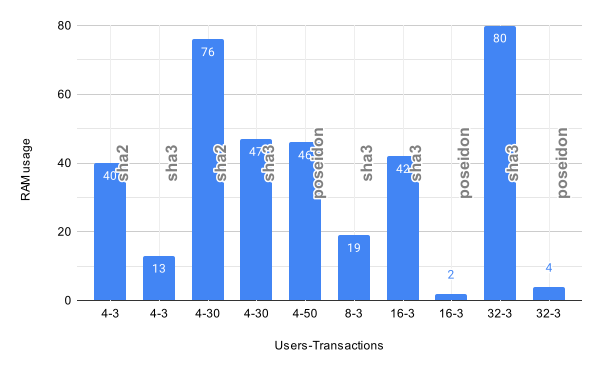
\includegraphics[width=0.7\columnwidth]{6_sheets-benchmarks_hash.png}
	\caption[RAM Usage hash]{RAM Requirements for each hash type.}  
	\label{fig:6_sheets-benchmarks_hash.png}
  \end{figure} 

\subsection{ZoKrates Rollup Performance\label{subsec:6_zokratesperf}}

A problem that emerges immediately when compiling the ZoKrates programs are the computational requirements to be able to compute the witness and generate a proof to submit to the Layer 1. The usage of the Poseidon hash function allowed the compilation of larger programs with more users and more transactions. Figure \ref{fig:6_sheets-resources-requirements.png} shows the RAM resources needed for the compilation phase of the rollup program. Note that the compilation phase is done only once, and the computation of the witness and generation of the proof are much less demanding, but those results show the complexity growth when adding transactions compared to adding users. This behavior is due to the fact that the verification of the signature still uses the sha2-256 hash function.

\begin{figure}[ht]
	\centering
	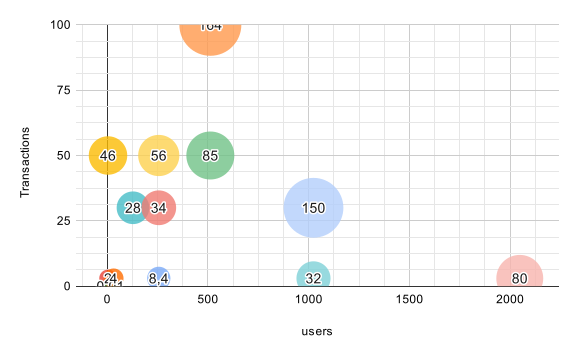
\includegraphics[width=0.7\columnwidth]{6_sheets-resources-requirements.png}
	\caption[RAM Requirements]{RAM Requirements for the compilation phase.}  
	\label{fig:6_sheets-resources-requirements.png}
  \end{figure} 

\subsection{Tezos Rollup Fees}

The verification performed by the verifier contracts and the subsequent update of the storage have costs. The verification cost is proportional to the size of the proof: during the proof verification, in fact, all the constraints are checked in a loop, consuming gas for each constraint verified. A single normal transaction between two users, as of 18/08/2023 costs 0.000518 tz.

Figure \ref{fig:6_sheets-cost-comparison.png} shows the fees for a single transaction in different scenarios of Rollup System size. The fees are calculated by submitting a rollup execution proof and looking at the fees payed for the proof verification and the storage update. The size of the bubble represent a visual amount of cost per transaction. From the graph is evident that even with a small Rollup System, the fees are very low, and they are always below the fees of a single transaction on the blockchain. Fees increase only with the increase number of transactions, due to the proof compression and reduction explained in Section \ref{sec:5_redandcompr}.

\begin{figure}[ht]
	\centering
	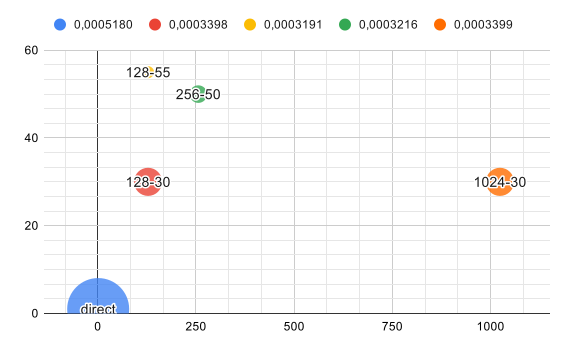
\includegraphics[width=0.7\columnwidth]{6_sheets-cost-comparison.png}
	\caption[Cost Comparison]{Cost per Transaction using different proof sizes.}  
	\label{fig:6_sheets-cost-comparison.png}
  \end{figure} 

  \section{Cost Model}

The proposed Rollup System has demonstrated greater efficiency compared to the conventional Layer 1 transaction system. However, there are additional costs that must be considered, including the expenses associated with running Layer 2 servers and the fees required for submitting and verifying proofs. In the current design, these costs are borne by the server initiating the proof. Consequently, the introduction of a fee system for Layer 2 users becomes necessary. It's important to highlight that inactive users on Layer 2 can be problematic, as they inflate the user list, thus increasing the operational costs of the entire rollup system. To address this issue, the implementation of a fee system is warranted.

\subsection{Fee System}

In order to execute a rollup, it is necessary to retrieve all users to recalculate the new Merkle root and determine the updated balances. As the number of users registering with the system increases, this process becomes slower. ZoKrates programs are capable of handling only powers of 2 numbers of users (including empty users) due to the merkle tree's structural characteristics. This can lead to exponential growth even when the number of users increases by just one.

Upon registering with the rollup system, a user transfers funds from their account to the Manager Smart Contract. This arrangement empowers the Manager Smart Contract to manage user funds by applying fees under specific circumstances. A proposed Fee Model revolves around the concept of a user's last activity, denoting the most recent instance of sending or receiving a transaction within the Rollup System. This information can be easily computed by the Manager Smart Contract while updating balances and nonces for senders and receivers after a successful proof verification.

An external server node may periodically retrieve the user list and identify stale accounts. Through a ZoKrates program that is subsequently verified, the server can compute the updated balances while levying fees on stale accounts. These fees can then be directly transferred to the Rollup Manager Smart Contract, which can utilize them to cover the costs of proof verification and storage updates.

\subsection{Reward System}

Layer 2 Rollup servers consist of two types: Web-Managers and ZoKrates executors. Web-Managers are economical servers, capable of operating with modest hardware specifications. They function as Docker containers hosting a database and node server. On the other hand, ZoKrates executors are relatively more resource-intensive, requiring a significant amount of RAM for witness computation and proof generation. However, ZoKrates executors possess an advantage: they need not run continuously, being solely necessary when computing and submitting proofs to the blockchain. This enables them to be deployed on a cloud service, activated only as needed. This approach effectively reduces the costs of Layer 2 operations while still necessitating a reward system.

Similar to the role of bakers in the Tezos blockchain when generating blocks, Layer 2 nodes can be rewarded for their contributions in submitting valid proofs. These rewards are extracted from the sender's balance during a transaction. The rewarded amounts are then attributed directly to the Rollup Manager Smart Contract's Layer 1 balance, enabling it to cover the costs of proof verification and storage updates without requiring modifications to the balance Merkle Tree.
    \chapter{Conclusion\label{cha:chapter7}}
% The final chapter summarizes the thesis. The first subsection outlines the main ideas behind Component X and recapitulates the work steps. Issues that remained unsolved are then described. Finally the potential of the proposed solution and future work is surveyed in an outlook.
% Explain what you did during the last 6 month on 1 or 2 pages!

\section{Summary\label{sec:summary}}

The work done in this master thesis allowed to show how a problem such as high transactions fee in the blockchain can be solved, by introducing a new layer on top of the blockchain, called Layer 2. The solution proposed has a simple architecture and can run on different blockchains with a few changes on the Layer 1. The system proposed is also capable of handling different types of token, like in the case of an NFT marketplace. Those results are compliant with the requirements of the project, described at \ref{cha:chapter3}, where is given remarkable importance to the need of having a system easily adaptable to different purposes.

\noindent The work done can be summarized into the following work steps:
\vspace{-0.11in}
\begin{itemize}
	\item Analysis of the already existing Zk-Rollup projects and solutions they provided to common problems;
	      \vspace{-0.11in}
	\item Analysis of the Tezos blockchain available functionalities and limitations;
	      \vspace{-0.11in}
	\item Analysis of ZoKrates toolbox and programs;
	      \vspace{-0.11in}
	\item Design and implementation of missing functionalities of Layer 2;
	      \vspace{-0.11in}
	\item Design and implementation of enhancements to L2;
	      \vspace{-0.11in}
	\item Design and implementation of a new and more efficient L1 to support the new L2;
	      \vspace{-0.11in}
	\item Benchmarking of the system, as single components and as a whole;
	      \vspace{-0.11in}
	\item Evaluation of the Rollup System.
\end{itemize}

The final Rollup System is capable of handling a good amount of users, tested in our system up to 2024, and a reasonable amount of transaction compared to the number of users, tested up to 55 transactions per rollup. From our tests emerged that the fee per single transaction executed in the Rollup System is reduced by 40\% compared to a normal L1 transaction and it gets linearly cheaper as more transactions are included in the rollup.

Witness and proof generation time are heavily dependant of the underlying CPU hardware running the ZoKrates program. Using our test environment it took a maximum of 40 minutes to generate a witness and proof for 1024 users and 30 transactions. This long execution time can be mitigated by using a more powerful CPU exploiting Cloud Services for small bursts of computation. Compared to the alternative rollup solution Optimistic Rollups, described at \ref{subsec:optimisticRollups}, our Zk-Rollup system has an incredibly lower confirmation period.

% \section{Dissemination\label{sec:dissemination}}

% Who uses your component or who will use it? Industry projects, EU projects, open source...? Is it integrated into a larger environment? Did you publish any papers?

\section{Problems Faced}

Some problems preventing the system to be functional were encountered during the development of the project. This is a brief overview to the most important.

\textbf{Hash Function}: the hash function revealed to be a critical  decision for reducing the hardware resources needed. From the initial sha2-256 hash function, we moved to Poseidon hash, with a 10000\% reduction in terms of RAM usage. This allowed to run the system from an initial version with 8 users, up to 2024 users.

\textbf{Proof Reduction and Compression}: as users were increasing in the Rollup System, the proof size was increasing too. This was preventing the proof to be sent to the verifier smart contract. To solve this issue, a proof reduction and compression algorithm was implemented, reducing the proof length from \textit{\#users*2} to \textit{\#transactions}. Although this approach works from Layer 2 side and verification phase, it is not yet possible to extract the compressed data to update the L1 storage due to missing functionalities in the SmartPy library.

\textbf{Repeated transition Attack}: malevolent users could send the same transaction multiple times, draining sender's account even if the transaction was properly signed. To solve this issue, a nonce was added to the transaction, preventing the same transaction to be executed more than once as the nonce has to be incremented at each transaction, allowing the system to check if the transaction has already been executed.

% Summarize the main problems. How did you solve them? Why didn't you solve them?

% \section{Outlook\label{sec:outlook}}
\section{Future Work}

Future work should be focused on the following points:

\vspace{-0.11in}
\begin{itemize}
	\item \textbf{Proof Reduction and Compression}: the proof reduction and compression algorithm should be completed on the Layer 1 to allow the system to update contract storage with the new balances and tokens.
	      \vspace{-0.11in}
	\item \textbf{Rollup System Optimization}: the Rollup System should be optimized to reduce the time needed to generate the witness and proof. This can be done by optimizing the ZoKrates program, or by evaluating performances on different CPU types and architectures;
	\item \textbf{Rollup System cost}: the costs of running the infrastructure should be studied to evaluate a fair transaction fee to apply to users to be able to reward nodes submitting valid proofs.
\end{itemize}


% Future work will enhance Component X with new services and features that can be used ...

    \chapter{Conclusion\label{cha:chapter8}}
% The final chapter summarizes the thesis. The first subsection outlines the main ideas behind Component X and recapitulates the work steps. Issues that remained unsolved are then described. Finally the potential of the proposed solution and future work is surveyed in an outlook.
% Explain what you did during the last 6 month on 1 or 2 pages!

\section{Summary\label{sec:summary}}

The work done in this master thesis allowed to show how a problem such as high transactions fee in the blockchain can be solved, by introducing a new layer on top of the blockchain, called Layer 2. The proposed solution presents a simple architecture adaptable to various blockchains with minimal adjustments to Layer 1. In particular, the system can accommodate diverse token types, including non-fungible tokens (NFTs), like in the case of an NFT marketplace. These achievements align with the project's requirements outlined in Chapter \ref{cha:chapter4}, where is given remarkable importance to the need of having an easily adaptable system.

\noindent The work can be summarized into the following work steps:
\vspace{-0.11in}
\begin{itemize}
	\item Analysis of existing Zk-Rollup projects and their solutions to common problems;
	      \vspace{-0.11in}
	\item Examination of functionalities and limitations of the Tezos blockchain;
	      \vspace{-0.11in}
	\item Study of ZoKrates toolbox and programs;
	      \vspace{-0.11in}
	\item Design and implementation of Layer 2 functionalities;
	      \vspace{-0.11in}
	\item Implementation of enhancements to Layer 2;
	      \vspace{-0.11in}
	\item Development of an efficient Layer 1 to support the new Layer 2;
	      \vspace{-0.11in}
	\item Benchmarking of single components and the entire system;
	      \vspace{-0.11in}
	\item Evaluation of the Rollup System.
\end{itemize}

The final Rollup System is capable of handling a considerable user load, tested up to 2024, and a proportional volume of transactions, tested up to 55 transactions per rollup. Results indicate a 40\% reduction in transaction fees per transaction compared to normal Layer 1 transactions, with costs decreasing linearly as transactions are included within the rollup.

Witness and proof generation times heavily depend on the underlying CPU hardware running ZoKrates. Test results showed a maximum of 40 minutes for generating a witness and proof for 1024 users and 30 transactions. Reduction of these extended execution times can be achieved through more powerful CPUs, leveraging cloud services for short bursts of computation. Notably, when compared to the alternative Optimistic Rollup solution, our Zk-Rollup system boasts significantly lower confirmation periods.

\section{Challenges Faced}

Several challenges were encountered during the project's progression, preventing its full functionality. The most important among these challenges are:
\vspace{-0.11in}
\paragraph{Hash Function} The choice of hash function revealed to be critical in hardware resource reduction. Transitioning from sha2-256 to Poseidon hash allowed a remarkable 10000\% decrease in RAM usage. This achievement allowed to run the system for a wider number of users, from an initial 8 users to up to 2024 users.
\vspace{-0.11in}
\paragraph{Proof Reduction and Compression} As user numbers grew, so did proof sizes, preventing its upload to the verifier smart contract. To solve this issue, a proof reduction and compression algorithm was implemented, reducing proof length from \textit{\#users*2} to \textit{\#transactions}. Although this approach works from Layer 2 side and verification phase, it is not yet possible to extract the compressed data to update the L1 storage due to missing functionalities in the SmartPy library.
\vspace{-0.11in}
\paragraph{Repeated Transition Attack} Malicious users could send repeated transactions, draining sender's account even with valid signatures. To counteract this, a nonce mechanism was introduced, preventing the same transaction to be executed more than once through nonce increment, allowing the system to check if the transaction has already been executed.

\section{Broad Usage\label{sec:dissemination}}

This project successfully proved the feasibility of implementing a Tezos-based Zk-Rollup system using the ZoKrates toolbox. The system's cost efficiency is superior than conventional L1 transactions, with the possibility to apply the system to different token types, like in the case of an NFT marketplaces. This versatility allows projects with different scopes to adopt the system in various blockchains and applications, requiring modest hardware capabilities, proportional of the amount of users and transactions foreseen in the application.

\section{Future Work}

The prototype developed in this thesis is an initial step towards a fully functional Zk-Rollup system. At the moment of writing, only the missing casting functionality in SmartPy, used during decompression, is preventing the system to be functional with high amount of users. Future work is needed to have and efficient and fully functional system. It should prioritize the following areas:
\vspace{-0.11in}
\begin{itemize}
	\item \textbf{Proof Decompression}: Complete the proof decompression algorithm for Layer 1 when the functionality will be available, allowing contract storage updates with new balances and tokens;
	      \vspace{-0.11in}
	\item \textbf{Rollup System Optimization}: Optimize the Rollup System to reduce witness and proof generation times. This can be achieved by ZoKrates program optimization and performance evaluations on different CPU types and architectures;
	      \vspace{-0.11in}
	\item \textbf{Rollup System Cost}: Study infrastructure operation costs to evaluate a fair transaction fee to reward nodes submitting valid proofs;
	      \vspace{-0.11in}
	\item \textbf{Stale user fee}: Study a fair fee amount for stale user, applying the algorithm described in Section \ref{subsec:7_staleuserfee}.
	\vspace{-0.11in}
\end{itemize}




% Future work will enhance Component X with new services and features that can be used ...

% ---------------------------------------------------------------
\backmatter % no page numbering from here
		
		% if you want to provide a glossary with explanations of important terms put it in here

    \bibliographystyle{geralpha}
    \bibliography{./bib/manual}
    
\end{document}
